\documentclass[10pt,a4paper]{article}
\usepackage[utf8]{inputenc}
\usepackage{amsmath}
\usepackage{amsfonts}
\usepackage{amssymb}
\usepackage{graphicx}
\usepackage{fancyhdr}
\pagestyle{fancy}
\fancyhead{}
\fancyhead[L]{\slshape MCTS Mario}
\fancyhead[R]{\slshape IT University of Copenhagen}
\fancyfoot{}
\fancyfoot[C]{\thepage}
%\graphicspath{ {C:\Users\Rasmus\workspace\MCTSMario\Rapport} }

\begin{document}
\title{Enhancements for Monte Carlo Tree Search in The Mario AI Framework}
\date{May 22, 2013}
\author{Emil Juul Jacobsen\\\texttt{ejuu@itu.dk}        
        \and Rasmus Greve\\\texttt{ragr@itu.dk}}
%TODO    \and \emph{Supervisor:}\\Julian Togelius\\\texttt{juto@itu.dk}}
\maketitle
\thispagestyle{empty} %Removes default pagenumber from frontpage

\begin{abstract}
(Bare copy/paste-ish fra projektbasen, skal skrives om!) %TODO
In this experiment we explore different implementations and enhancements of the Monte Carlo Tree Search algorithm for an AI, in order to evaluate their performance and results in the Super Mario AI Benchmark tool. 
We have implemented the basic MCTS algorithm in the Mario AI 
Framework and characterised the performance and identification of 
the strengths and weaknesses of the algorithm relative to the 
framework. We have identified a set of refinements and alterations of the algorithm 
and through implementation and evaluation of these individually we came up
with compositions that greatly increase the performance of the AI.
\end{abstract}
\clearpage

\section{Introduction}
In this experiment we explore different implementations and enhancements of the Monte Carlo Tree Search (MCTS) algorithm for an AI, in order to evaluate their performance and results in the Super Mario AI Benchmark tool. The MCTS algorithm has shown great results in various classical board games but has (to our knowledge) not been tested on a real-time physics-based game like Super Mario. Like some of the games that MCTS has proven effective in, Super Mario has a great branching factor of the state space but differs in that simulating actions is quite computationally heavy. These differences make several modifications of the core algorithm interesting for our experiment because they can help build the tree in a manner that uses the simulations more effectively. %TODO
\clearpage

\section{Background}
%TODO Fill this space
\subsection{Monte Carlo Tree Search}
Monte Carlo Tree Search has shown surprisingly good results in solving problems with large branching factors. MCTS is a tree search algorithm, where evaluation of a node is done by random sampling in the decision space until an outcome can be determined. A very nice quality of MCTS is that it is an \emph{anytime} algorithm, meaning that it can be halted when a time budget is reached and give the result that looks the most promising at the given time. Furthermore it often requires no or very little domain knowledge as a naïve implementation only require knowledge of the action space and a means of simulating the outcome of an action. %TODO Not naive, something else!

Searching in MCTS is done by iteratively by building a search tree where the nodes are game states, and the edges are actions. A node is added to the tree in each iteration and based on the value of the new node, the values of parent nodes are updated.
An iteration of MCTS consists of four steps:
\begin{enumerate}
\item Selection (A node to be expanded is chosen)
\item Expansion (The node is expanded by simulating the associated action)
\item Simulation (The game is simulated with random moves until terminal)
\item Back propagation (The result propagates up through the tree)
\end{enumerate}

\subsection{Upper Confidence Bounds for Trees}
Choosing which node to expand can be done in multiple ways. Upper Confidence Bound (UCB) is a bandit based approach to choosing the most urgent node to expand. The quality with UCB is that it allows for prioritizing between exploration of less tried nodes, and exploitation of seemingly promising nodes.
\textbf{OBS! Præcis hvilken ligning skal vi skrive her????}
\begin{equation}
\label{eq:ucb1}
\displaystyle UCB_j = \overline{X}_j + \sqrt{\frac{2 * \log(n)}{n_j}}
\end{equation}
$X_j$ is the average (i.e. expected) reward. $n$ is the total number of plays and $n_j$ is the number of times action $j$ was tried.

\subsection{The Mario AI Framework}

\subsection{Enhancements and Improvements}

\begin{itemize}
\item Om MCTS \cite{mctssurvey}
\item Om UCB og UCT \cite{mctssurvey} måske også \cite{mspacman}
\item (kort!) Om The Mario AI Framework  \cite{mario}
\item Om forbedringer
\end{itemize}
\clearpage

\section{Approach and Enhancements}
In this section we will go over the different implementations and enhancements that we have experimented with. For enhancements including a value that can be tweaked we have tried finding the optimal setting, and in the end we have combined enhancements which complement each other well.

\subsection{Monte Carlo Tree Search with UCB}
To have a baseline for comparison and an implementation to build on, we started by implementing the basic Monte Carlo Tree Search algorithm with Upper Confidence Bounds for selection of nodes.
Source \cite{mctssurvey}
\subsection{Domain knowledge}
While MCTS on it's own does show some intelligent behaviour, we felt like we had to introduce some domain knowledge to the algorithm to make it perform better. Otherwise most of the enhancements to make wouldn't really show much difference, as it in any case would lead to quite a large amount of random behaviour.

\subsubsection{Limited actions}

%TODO Down button

The absolute first piece of domain knowledge that we introduced was to remove the possibility of pressing the down arrow making Mario duck. In a very few cases it indeed does make sense to duck - under a bullet or a flying monster - but while it can be of use, it also doubles the action space from 16 to 32 possible actions which reduces the reachable depth significantly.
Another important factor that made us disable the down button was that while the down button is pressed, pressing left or right does not make Mario move. %TODO 

%TODO Specific actions

Hvis vi er nødt til at begrænse ham til ikke at bruge $\downarrow$ til alle de andre implementationer skal det fremgå her!
\subsubsection{Hole detection}
Hvis vi er nødt til at bruge hulgenkendelse til alle de andre implementationer skal det fremgå her!
\subsection{Softmax Backup}
\begin{equation}\label{eq:softmax_equation}
exploitation = Q * maxReward + (1 - Q ) * averageReward
\end{equation}
We use equation \ref{eq:softmax_equation} to calculate the exploration part for the confidence of nodes
\subsection{Macro actions}
\cite{salesman}
\subsection{Heuristic Partial Tree Expansion Policy}
\subsection{Checkpoints}
\subsection{(Combination)}
\clearpage

\section{Results}
\renewcommand{\arraystretch}{1.5}
\begin{table}[h]
	\centering
	\begin{tabular}{| l | l |}
		\hline
		\textbf{Method} & \textbf{Score} \\ \hline
		Softmax backup q = 0 (UCT) & 34,162 \\ \hline
		Softmax backup q = $\frac{1}{8}$ & - \\ \hline
		Softmax backup q = $\frac{1}{4}$ & 34,387 \\ \hline
		Softmax backup q = $\frac{1}{2}$ & 34,147 \\ \hline
		Softmax backup q = 1 & 26,842 \\ \hline
	\end{tabular}
	\caption{Results of using Softmax backup with different q values}
	\label{tab:softmax_results}
\end{table}
\begin{table}[h]
	\centering
	\begin{tabular}{| l | l | l |}
		\hline
		\textbf{Method} & \textbf{Avg. number of nodes} & \textbf{Score} \\ \hline
		MCTS w/ UCT, limit = 0			& - & - \\ \hline
		MCTS w/ UCT, limit = 1			& - & - \\ \hline
		MCTS w/ UCT, limit = 2			& - & - \\ \hline
		MCTS w/ UCT, limit = 4			& - & - \\ \hline
		MCTS w/ UCT, limit = 8			& - & - \\ \hline
		MCTS w/ UCT, limit = 16			& - & - \\ \hline
		MCTS w/ UCT, limit = $\infty$	& - & - \\ \hline
	\end{tabular}
	\caption{Results of using UCT with a different limit for random moves}
	\label{tab:uct_results}
\end{table}
\begin{figure}[h]
\centering
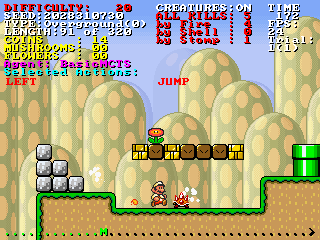
\includegraphics[width=6cm]{Forfulgt.png}
\caption{Mario being followed}
\label{fig:followed}
\end{figure}
Her er noget mere tekst, reference til figur \ref{fig:followed}
\clearpage
\section{Conclusion}
\clearpage

\begin{thebibliography}{9}
\bibitem{mctssurvey}
  C. B. Browne, E. Powley, D. Whitehouse, S. M. Lucas, P. I. Cowling, P. Rohlfshagen, S. Tavener, D. Perez, S. Samothrakis, and S. Colton, “A survey of monte carlo tree search methods,” Computational Intelligence and AI in Games, IEEE Transactions on, vol. 4, no. 1, pp. 1–43, 2012.

\bibitem{civii}
S. R. K. Branavan, D. Silver, and R. Barzilay, “Non-linear monte-carlo search in civilization ii,” in Proceedings of the Twenty-Second international joint conference on Artificial Intelligence-Volume Volume Three, 2011, pp. 2404–2410.

\bibitem{salesman}
E. J. Powley, D. Whitehouse, and P. I. Cowling, “Monte Carlo Tree Search with macro-actions and heuristic route planning for the Physical Travelling Salesman Problem,” in Computational Intelligence and Games (CIG), 2012 IEEE Conference on, 2012, pp. 234–241.

\bibitem{mspacman}
T. Pepels and M. H. Winands, “Enhancements for Monte-Carlo Tree Search in Ms Pac-Man,” in Computational Intelligence and Games (CIG), 2012 IEEE Conference on, 2012, pp. 265–272.

\bibitem{mario}
S. Karakovskiy and J. Togelius, “The mario ai benchmark and competitions,” Computational Intelligence and AI in Games, IEEE Transactions on, vol. 4, no. 1, pp. 55–67, 2012.
\end{thebibliography}

\end{document}